\documentclass[12pt,preprintnumbers,amsmath,amssymb,nofootinbib,superscriptaddress]{revtex4-1}
\usepackage[paperheight=12cm,top=0.5cm,bottom=0.5cm,left=1cm,right=1cm]{geometry}
\usepackage{xparse}
\NewDocumentCommand{\DIV}{om}{%
  \IfValueT{#1}{\setcounter{#2}{\numexpr#1-1\relax}}%
  \csname #2\endcsname
}

\usepackage[latin1]{inputenc}
\usepackage{slashed}
\usepackage{amsmath}
\usepackage{textcomp}
\usepackage{amssymb}
\usepackage{amsfonts}
\usepackage{indentfirst}
\usepackage{color}
\usepackage[dvipsnames]{xcolor}
\usepackage{hyperref}
\usepackage{subcaption}
\usepackage{graphicx,graphics}
\graphicspath{{figures/}}
\usepackage[skins,theorems,many]{tcolorbox}
\tcbset{highlight math style={enhanced,
  colframe=red,colback=white,arc=0pt,boxrule=1pt}}
\usepackage[abs]{overpic}
\usepackage{xcolor,varwidth}
\usepackage[english]{babel}
\usepackage{blindtext,tikz}
\usetikzlibrary{calc}
\usepackage{fancyhdr}
\usepackage{eso-pic}
\usepackage{csvsimple}
%\usepackage{pgfplotstable,filecontents}
%\pgfplotsset{compat=1.9}% supress warning
\usepackage{booktabs}


\long\gdef\@calc@trim< #1 >\@/< #2 >\@/< #3 >\@/< #4 >\@/< #5 >\@/< #6 >\@/< #7 >\@/< #8 >\@/< #9 >\@nihil{%
    \ifcase\numexpr2#3#8\relax\or#2\or#7\or#5\or#1\or#1\fi%
}

\long\gdef\trim#1{%
    \@calc@trim< #1 >\@/< #1>\@/< - >\@/< + >\@/< ? >\@/<#1 >\@/<#1>\@/< 0 >\@/< 2 >\@/< 1 >\@/< 3 >\@/< 2 >\@/< ! >\@nihil%
}


\def\bibsection{\section*{}} %Removes black line above refrences

%--------------------------%
%----- COLOURED BOXES -----%
%--------------------------%

%Blue equation box
%\tcbhighmath[colframe=RoyalBlue!70!black,colback=RoyalBlue!25!white]{

%Orange equation box
%\tcbhighmath[colframe=BurntOrange!95!black,colback=BurntOrange!45!white]{

%Purple equation box
%\tcbhighmath[colframe=Purple!150!black,colback=Purple!30!white]{

%Green equation box
%\tcbhighmath[colframe=ForestGreen,colback=ForestGreen!25!white]{

%Grey equation box
%\tcbhighmath[colframe=Black,colback=Black!10!white]{

%Pink equation box
%\tcbhighmath[colframe=magenta,colback=magenta!20!white]{

%Blue and red equation box
%\tcbhighmath[frame style={left color=RoyalBlue!70!black,right color=Red!95!black},interior style={left color=RoyalBlue!35!white,right color=Red!50!white}]{

%Red and green equation box
%\tcbhighmath[frame style={left color=Red!95!black,right color=ForestGreen},interior style={left color=Red!50!white,right color=ForestGreen!25!white}]{

% ---------------------------------------------------------

\begin{document}
\pagenumbering{gobble}

\begin{titlepage}
\hfill{}
\vspace{1.5cm}
\begin{center}
    % Add some 'virtue signaling' just to make Max upset
    \tcbhighmath[frame style image=report_images/grad.jpg,interior style image=report_images/title_interior.jpg, boxrule=2pt]{\text{\huge DD-MM-YYYY TELESCOPE-NAME}}
    \\[1cm]
    DINOS: Display Information Needed for Observing Stuff
    %\includegraphics[width=4cm]{Figures/toaster.jpg}
    \AddToShipoutPictureBG*{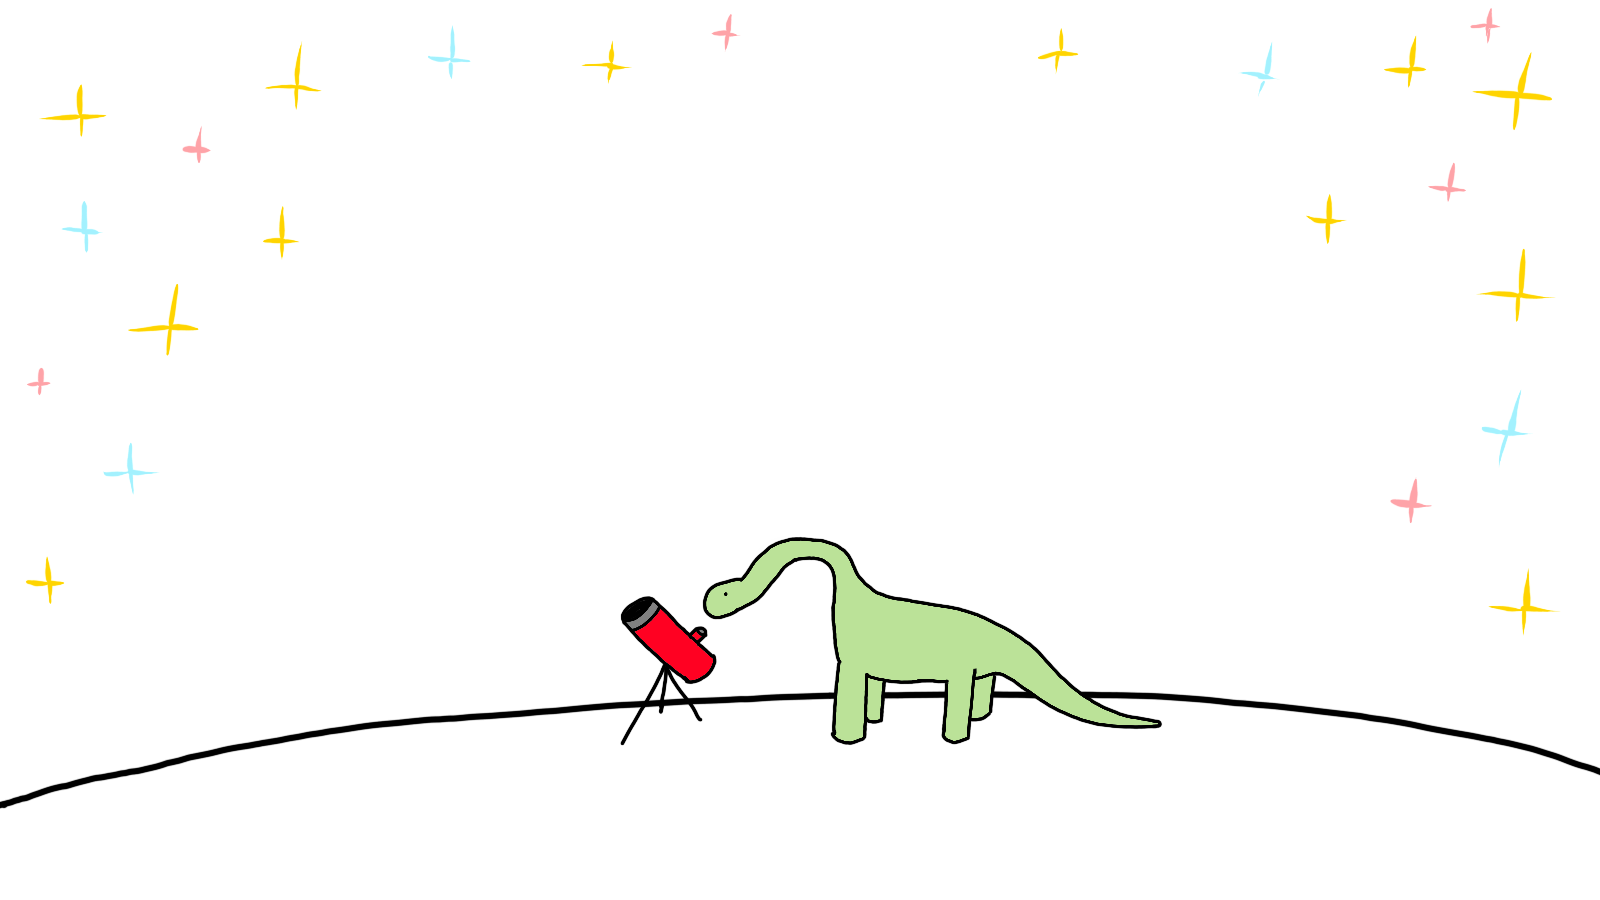
\includegraphics[width=\paperwidth,height=\paperheight]{report_images/titlebackground_v2.png}}
\end{center}
\end{titlepage}

%-----EXAMPLE SLIDES-----%
%THENIGHT
%\newpage

%\DIV[1]{section}*{The Night}\label{Ueff}
%\vspace{-0.2cm}\hrule
%\vspace{1cm}

%include information about location, sunrise/set, observing window, blocks, the telescope

%\newpage 

%\DIV[1]{section}*{Weather Report}\label{Ueff}
%\vspace{-0.2cm}\hrule
%\vspace{1cm}

\newpage

\DIV[1]{section}*{Targets}\label{Ueff}
\vspace{-0.2cm}\hrule
\vspace{1cm}

\begin{center}
\begin{tabular}{l|c|c|c|c|c|c}%
    \bfseries Object & \bfseries RA & \bfseries DEC & \bfseries Type & \bfseries Spectral Class & \bfseries Distance (kpc) & \bfseries Apparant V mag  % specify table head
    \csvreader[head to column names]{targets.csv}{} % use head of csv as column names
    {\\\hline\Object & \RA & \DEC & \oType & \spType & \d & \V} % specify your coloumns here
\end{tabular}

\end{center}

\newpage


\DIV[1]{section}*{All-Sky Map}\label{Ueff}
\vspace{-0.2cm}

\begin{center}
    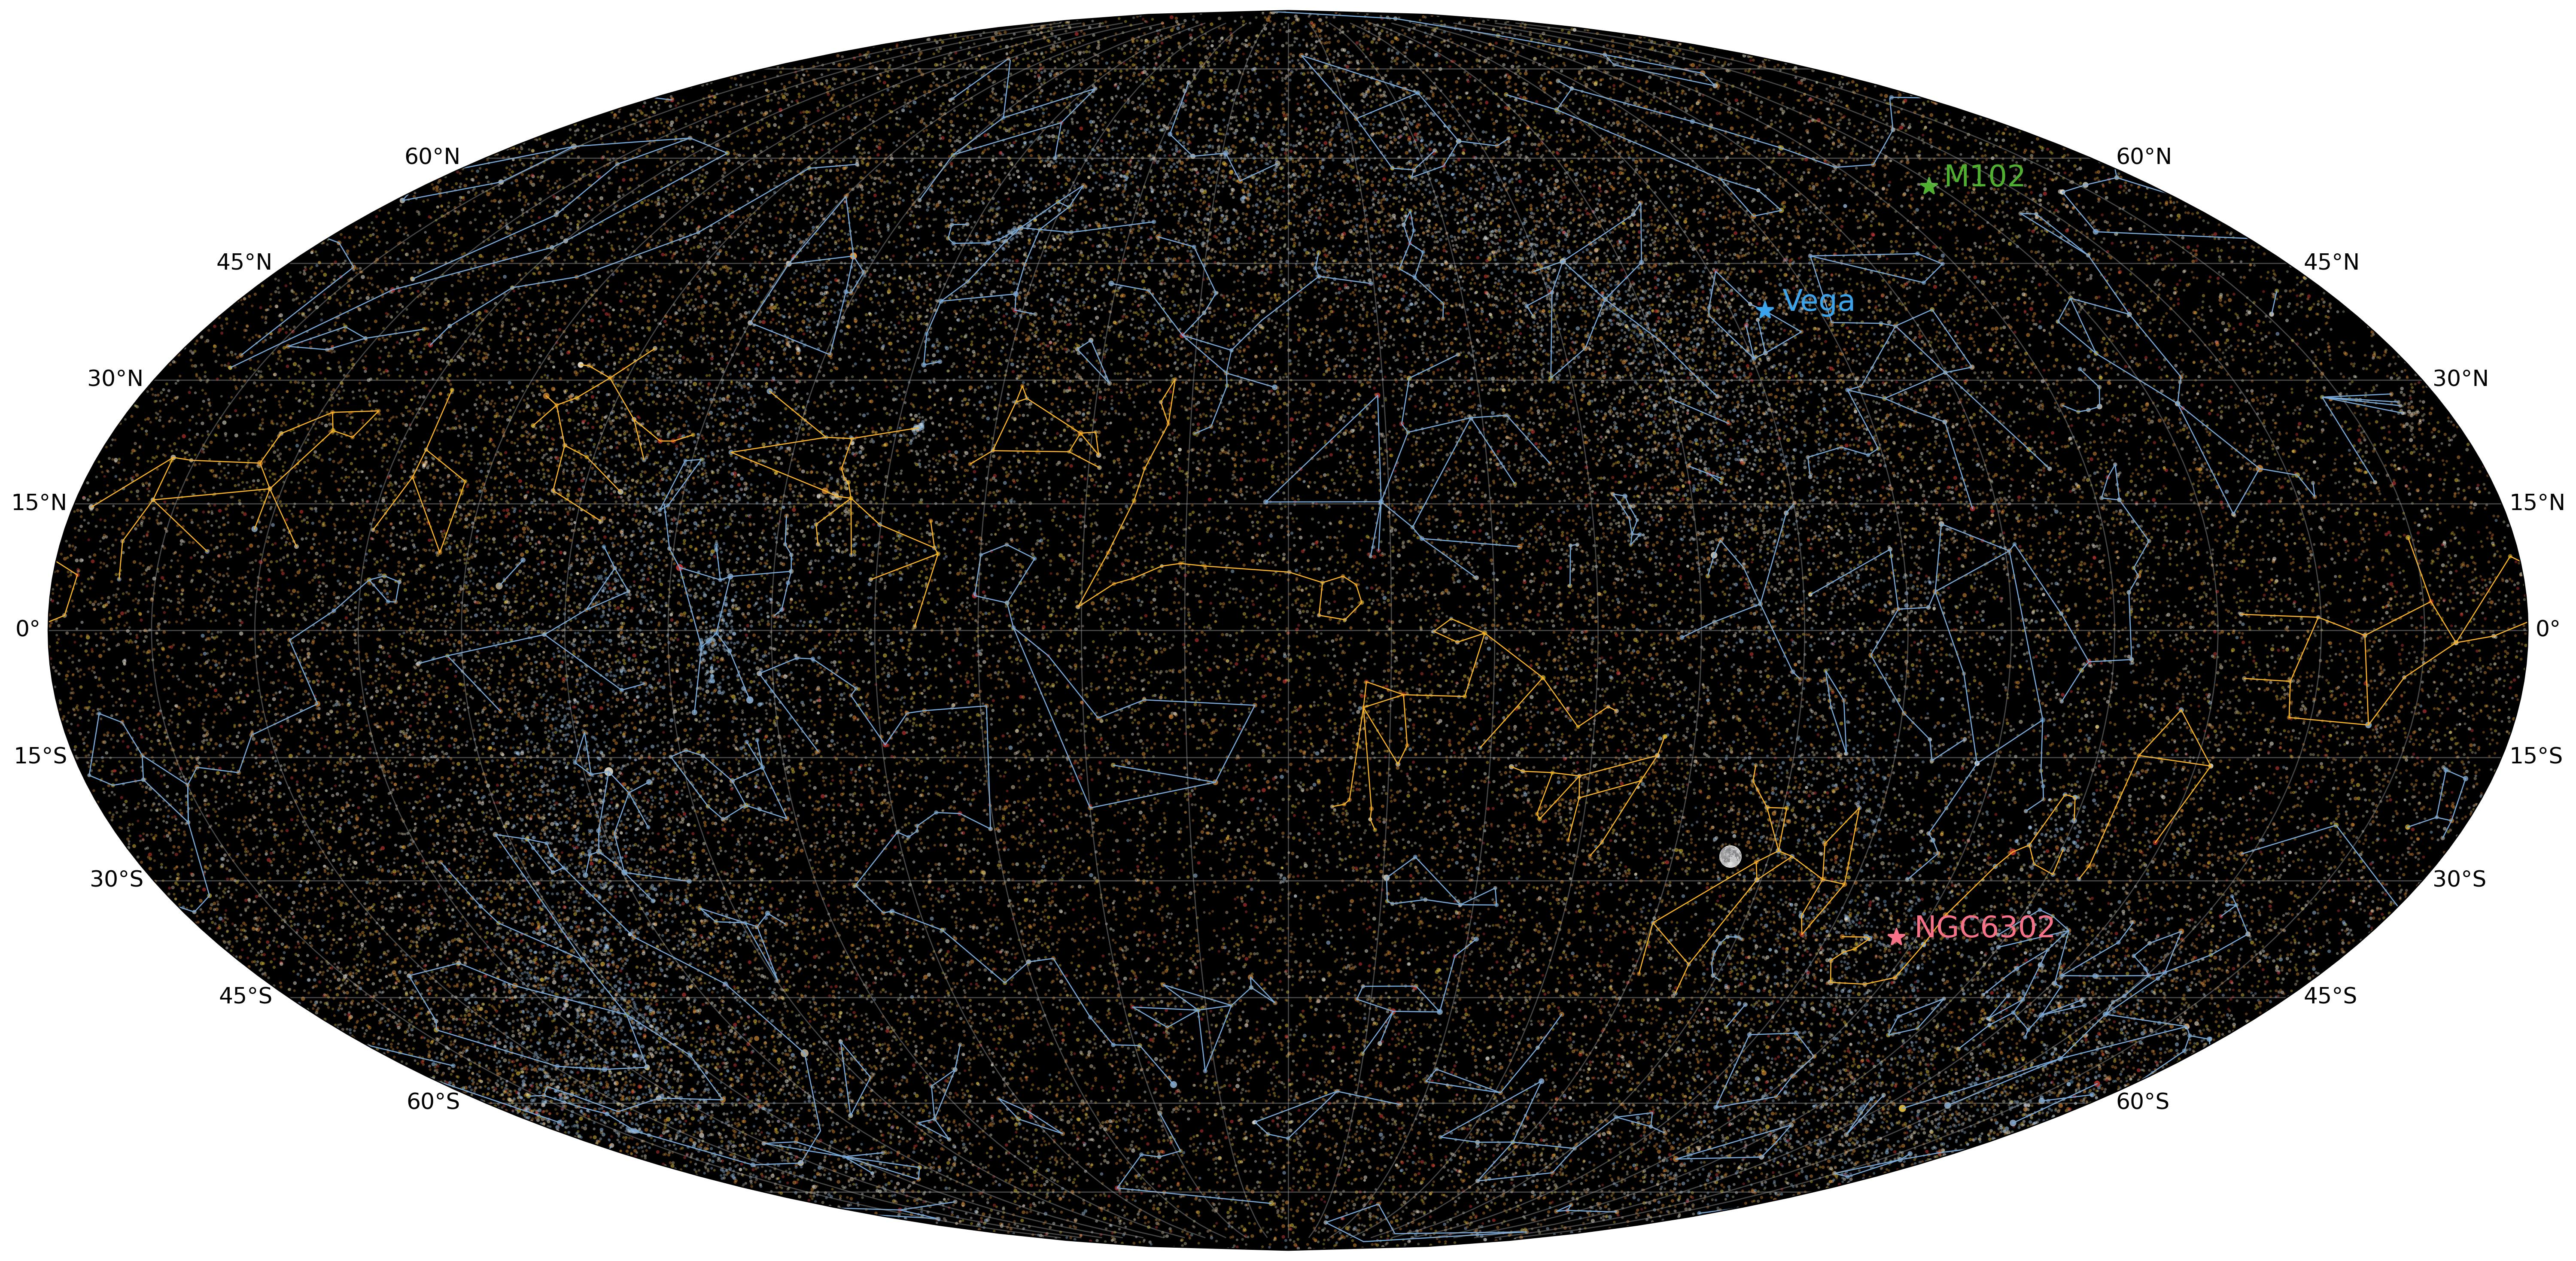
\includegraphics[width=1.0\textwidth]{OUTPUTDIRECTORY/all_sky_map.jpg}
\end{center}

\newpage

\DIV[1]{section}*{Local-Sky Plot}\label{Ueff}
\vspace{-0.2cm}

\begin{minipage}{0.6\textwidth}
    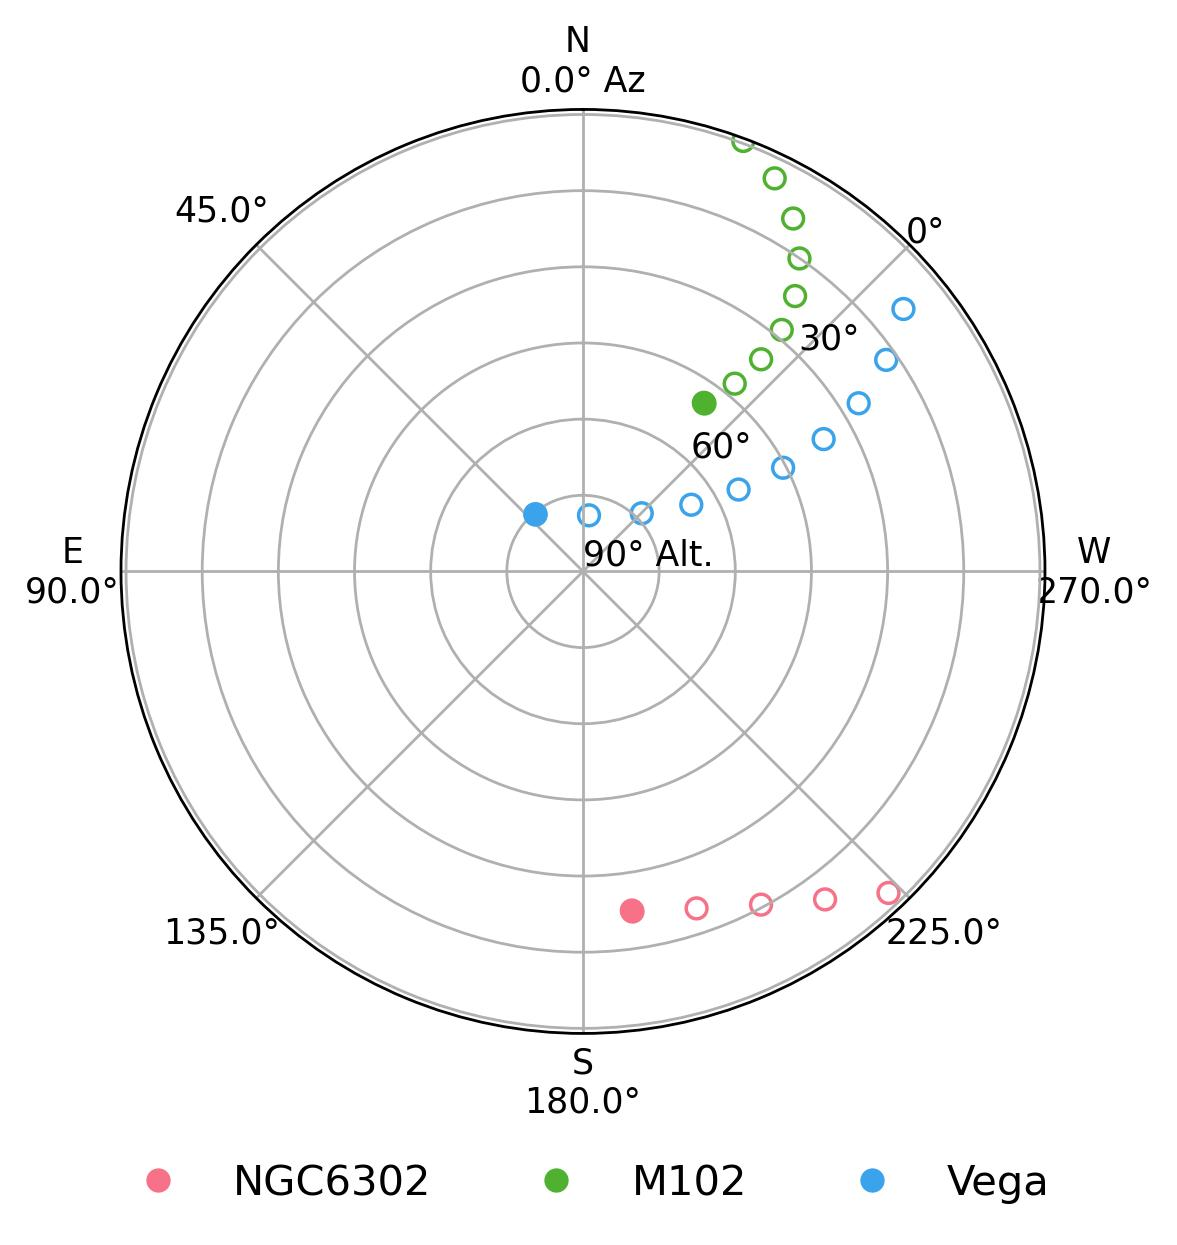
\includegraphics[width=9cm]{OUTPUTDIRECTORY/local_sky.jpg}
\vspace{-2cm}

\end{minipage}
\begin{minipage}{0.3\textwidth}

\begin{center}
\begin{tabular}{l|c|c}%
    \bfseries Object & \bfseries Rise Time & \bfseries Set Time   % specify table head
    \csvreader[head to column names]{targets.csv}{} % use head of csv as column names
    {\\\hline\Object & \rise & \set } % specify your coloumns here
\end{tabular}

\end{center}

\end{minipage}

\newpage 

\DIV[1]{section}*{Airmass Plot}\label{Ueff}
\vspace{-0.2cm}

\begin{center}
    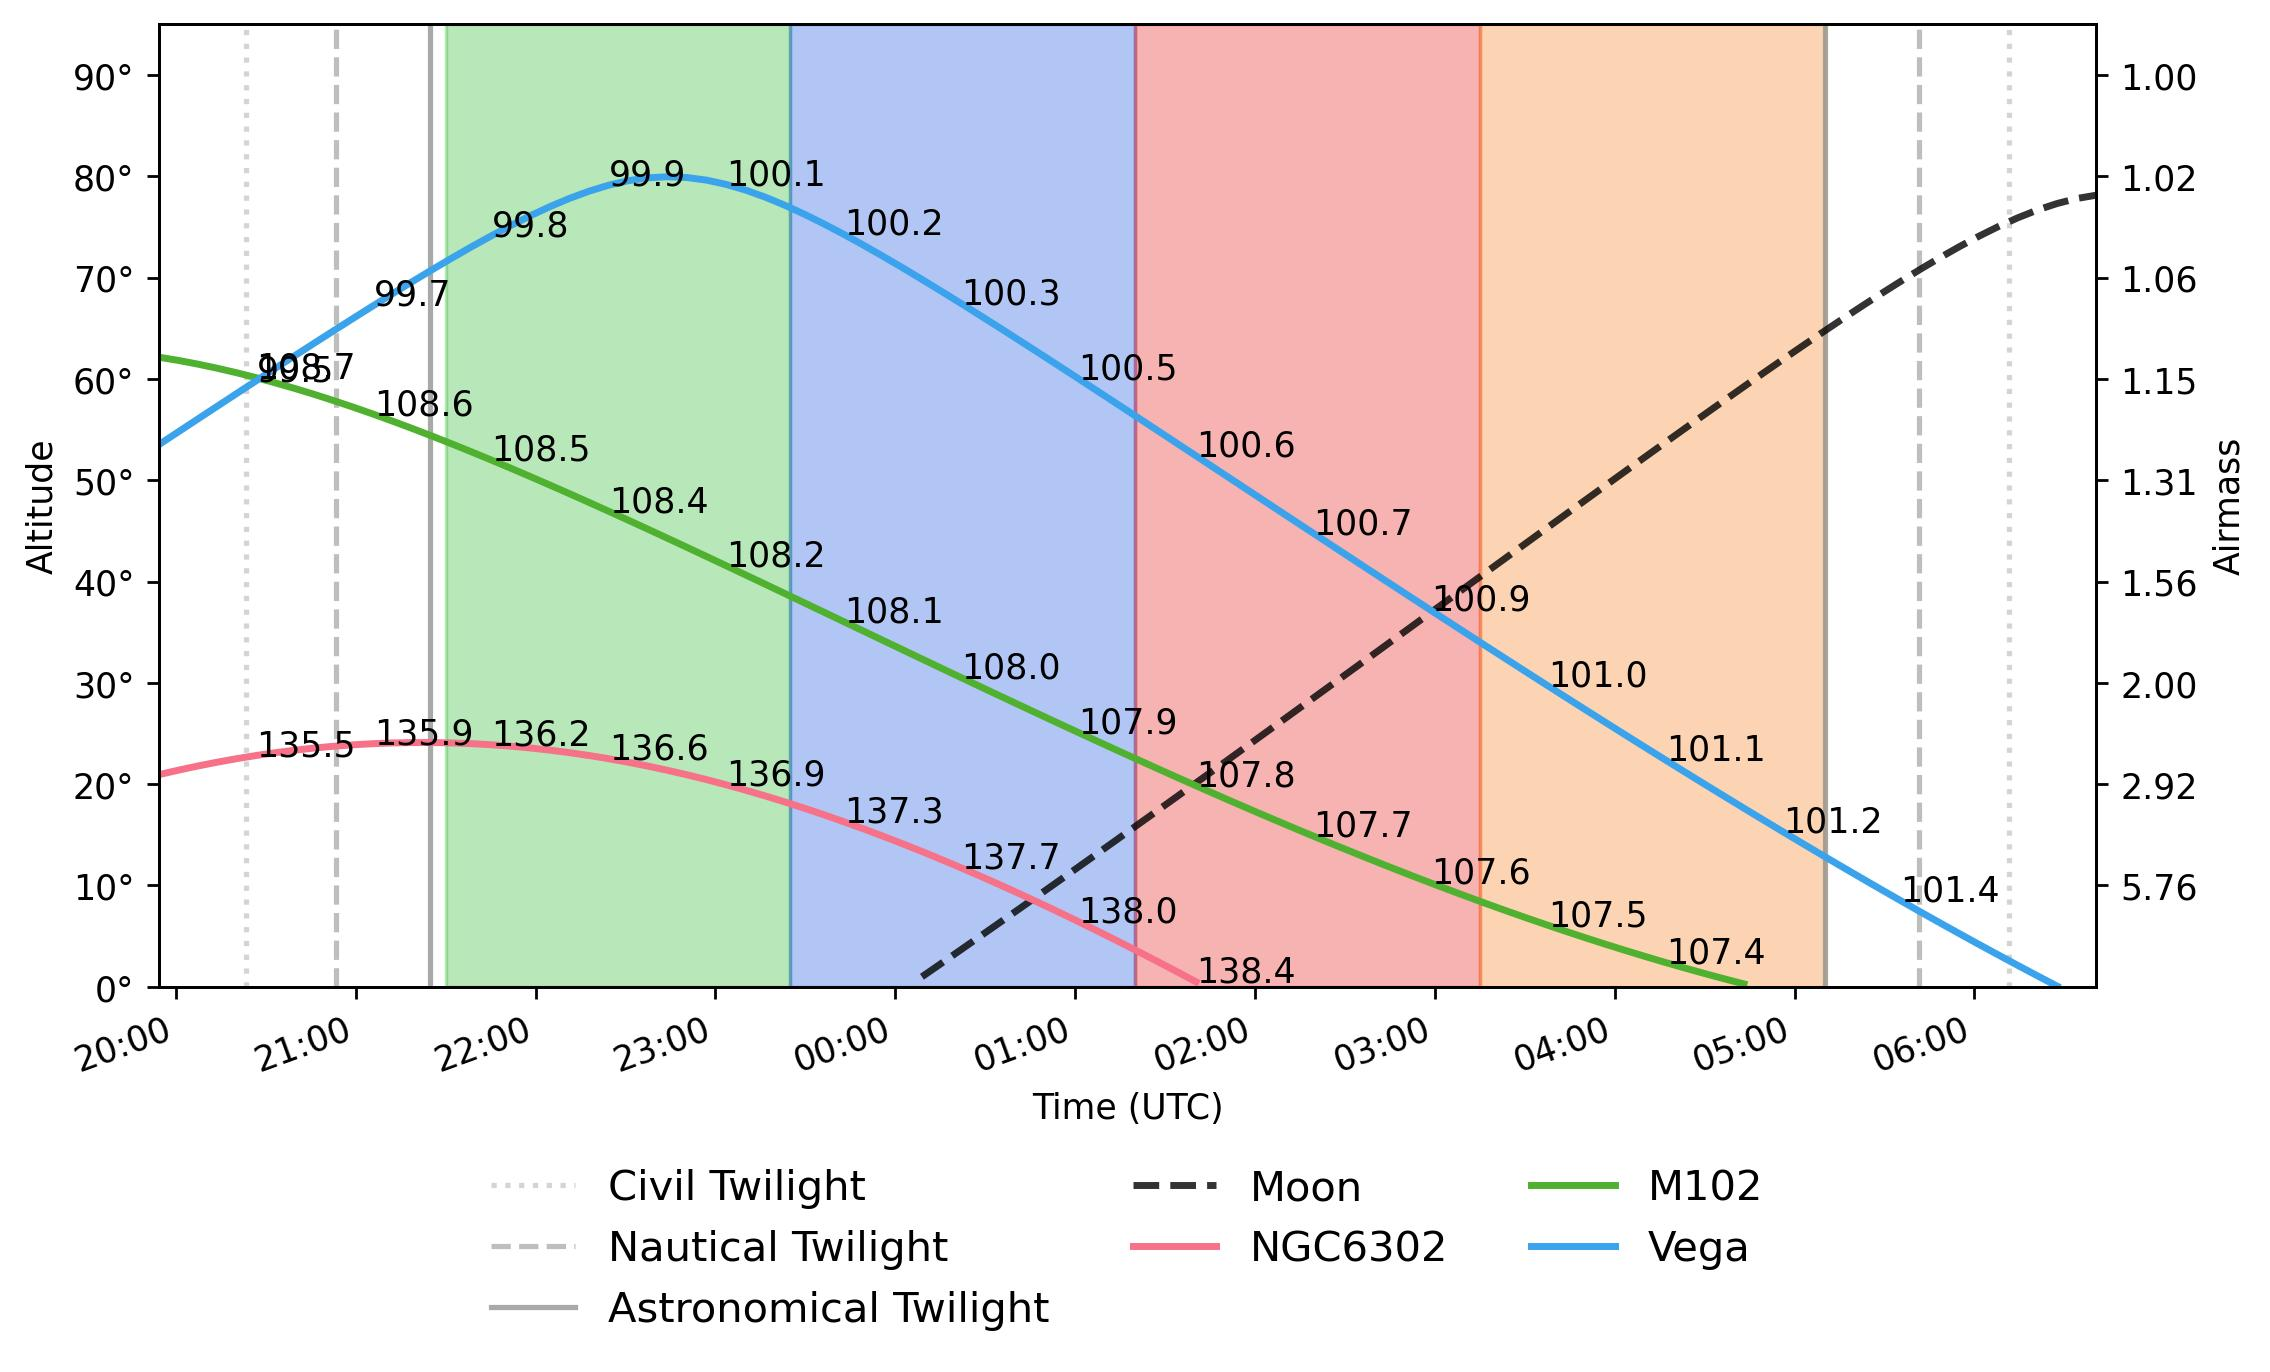
\includegraphics[width=0.75\textwidth]{OUTPUTDIRECTORY/airmass.jpg}
    \captionof*{figure}{\scriptsize Observing blocks are shown as the shaded regions. The numbers along each curve represent the angular distance between that target and the moon.}
\end{center}

%FINDERCHARTS

\newpage

\DIV[2]{section}*{Acknowledgements}
\vspace{-0.2cm}\hrule
\vspace{1cm}

DINOS was developed by Lars Borchert making use of open source software.
The LaTeX \href{https://www.overleaf.com/latex/templates/academic-presentation-template/jpgfpsstrwzd}{template} for this PDF was made by D. Backhouse.
The all-sky map was heavily inspired by \href{https://github.com/eleanorlutz/western_constellations_atlas_of_space}{Eleanor Lutz's} map of all the stars you can see from Earth, on GitHub.
The "rey" asterisms were developed by H.A. Rey for his book \href{https://en.wikipedia.org/wiki/The_Stars:_A_New_Way_to_See_Them}{"The Stars: A New Way to See Them"}.
The asterism files were taken from the open source planetarium software \href{https://stellarium.org/}{Stellarium}.
The DINOS terminal text was made using the text to ASCII art tool by \href{http://patorjk.com/software/taag/#p=display&f=Bi}{patorjk}.

\end{document}